\graphicspath{{Chapter_5_-_Code_structure/Images/}}
\chapter{Code structure}
\quad\, In the chapter \ref{Brayton cycle}, the Brayton cycle has been introduced by presenting two possible configurations 

This chapter will start from these notions to build a computer code simulating the performance of the Brayton cycle. The analysis will be performed in steady state operations and will not take into account transient effects. For instance, transient effects include the acceleration or deceleration analysis of the turbomachines, the modulation of the mass flow of fuel in the time, etc.

The computer code that will be presented during this chapter will be based on the Python language\citep{van1995python}. The motivations of the usage of this particular computing language, will be given in the beginning of this chapter. Then, the structure of the code itself will be established, followed by the method of implementation of the theoretical aspects from chapter \ref{C3}.

\section{Python language}
\quad\, Python is a computing language that was created by Guido van Rossum at the Centrum Wiskunde \& Informatica (CWI - \url{https://www.cwi.nl}) in the early 1990s. Starting 1995, G. van Rossum continued to work on Python at the Corporation for National Research Initiatives (CNRI - \url{https://www.cnri.reston.va.us/}). Since the very first release, the language was open source. This means that the source code was accessible to anyone. 

From this time, Python progressively gained in popularity, and the community participating to the development of the software didn't stop to grow. Today, this language is used by many companies and for many types of applications. Indeed, this programming language is used for website creation, machine learning, automation, etc. 

Since Python is an open source language, it lives thanks to its community which creates and shares libraries. Indeed, what have already been implemented in the past can be freely used by the other users. Moreover, new users can easily start developing under Python thanks to huge amount of guide and documentation to starting learning about the Python language.

Also, Python is a programming language that allows the object oriented programming. This paradigm consist in the definition of blocks of code (called objects) which are able to interact together through relations. These relations are defined in order to solve a given problem.

The usage of Python within the scope of this work has been motivated by the previously mentioned characteristics.

\section{Code structure}
\quad\, the previous section explained the motivations behind the choice of Python as programming language for the realization of this work.

In this work, a program aiming to simulate the steady state performance of a Brayton cycle considering various configurations. As a reminder, the base Brayton cycle is composed of the following transformations illustrated on Figure \ref{fig:C4_Brayton}:

\begin{itemize}
\setstretch{1}
\item Compression through a compressor (COMP)
\item Combustion within a combustion chamber (CC)
\item Expansion through a turbine (TURB)
\end{itemize}

\begin{figure}[h]
\centering
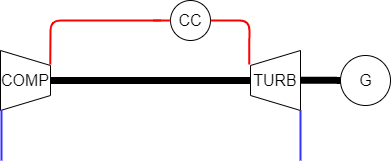
\includegraphics[width=0.5\textwidth]{GT}
\caption{Brayton gas turbine (GT)}
\label{fig:C4_Brayton}
\end{figure}

